\chapter{Wireframing}
\section{Smartphone}
The design for the smartphone consists of four different pages. 
\subsection{Login}
The login dialogue is the first page you see. There are two input fields for the username and the password. Below these input fields there is the login button to confirm and login. Then there is a radio button to stay logged in.

The link if the password has been forgotten and a button to register and create a new user account are the last things on this page.
\subsection{Menu}
The menu pops up from the left edge as you can see on the picture. It can be chosen between viewing the tracks, customize settings, view statistics and logout.
\subsection{Tracks}
On the tracks page a map shows the last track by default but on the bottom any available track can be chosen to view it.
\subsection{Settings}
Under settings, basically changes like edit the mail address or change the password of the account can be applied, but also if the default track type should be private or public.
\subsection{Statistics}
It’s possible to view a graph where informations of driven tracks are shown. Every registered car of this account can be chosen to view it’s graph and additionally, it’s selectable if the displayed data was tracked the last week, month or year.
\begin{center}
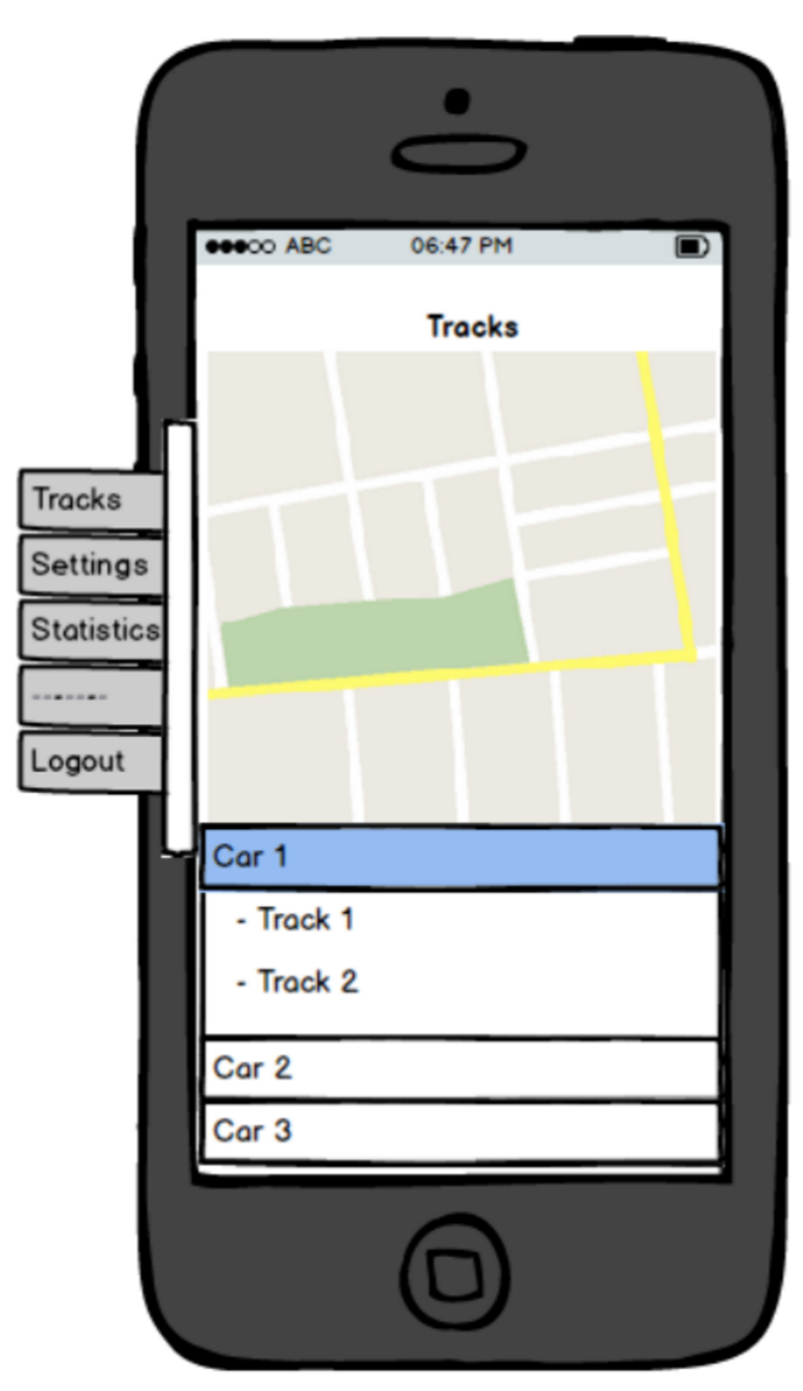
\includegraphics[width=0.4\textwidth]{bilder/Smartphone}
\end{center}
\section{Tablet}
The wireframing we created for the Tablet design is nearly similar to the smartphone design. Except of view extensions such as for renaming the device and editing tracks more precise.
\subsection{Login}
The login dialogue is the first page you see. There are two input fields for the username and the password. Below these input fields there is the login button to confirm and login. Then there is a radio button to stay logged in.
The link if the password has been forgotten and a button to register and create a new user account are the last things on this page.
\subsection{Menu}
The menu pops up from the left edge as you can see on the picture. It can be chosen between viewing the tracks, customize settings, view statistics, rename the device, register a car and logout.
\subsection{Tracks}
On the tracks page a map shows the last track by default. A track can be selected and there is the option to edit or merge a route.
\subsection{Settings}
Under settings, basically changes like edit the mail address or change the password of the account can be applied, but also if the default track type should be private or public.
\subsection{Rename Device}
Every device has a name and to know better which device is which, it is possible to give the devices names.
\subsection{Register Car}

\subsection{Statistics}
It’s possible to view a graph where informations of driven tracks are shown. Every registered car of this account can be chosen to view it’s graph and additionally, it’s selectable if the displayed data was tracked the last week, month or year.
\begin{center}
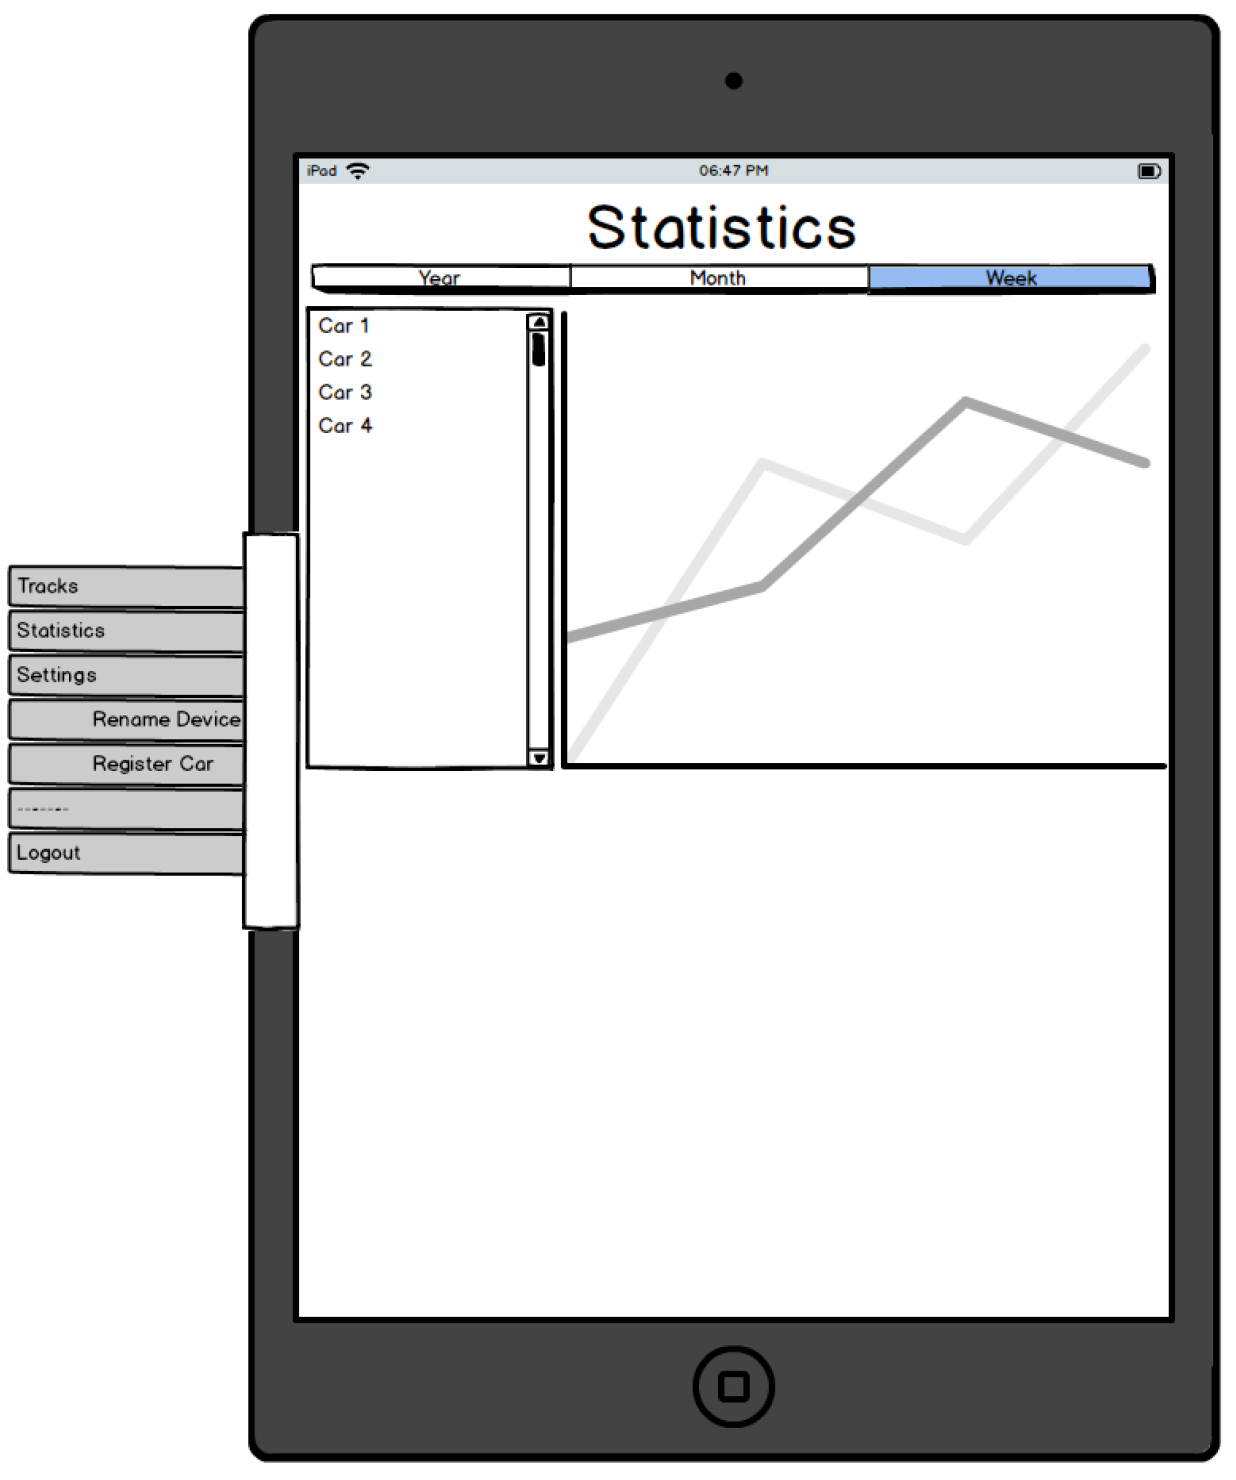
\includegraphics[width=0.625\textwidth]{bilder/Tablet}
\end{center}
\section{Web Portal}
\subsection{Home}
Before the user is logged in, information about the product is shown on this page.

After the login, all tracks are shown and it is possible to change the tracks from private to public.
\subsection{Login}
The login dialogue is the first page you see. There are two input fields for the username and the password. Below these input fields there is the login button to confirm and login. Then there is a radio button to stay logged in.
The link if the password has been forgotten and a button to register and create a new user account are the last things on this page.
\subsection{Settings}
Under settings, basically changes like edit the mail address or change the password of the account can be applied, but also if the default track type should be private or public.
\subsubsection{Register Car}

\subsubsection{Rename Device}
Every device has a name and to know better which device is which, it is possible to give the devices names.
\subsection{Track}
On the tracks page a map shows the last track by default. It can be chosen between the cars and the tracks of the respective cars can be viewed.
\subsubsection{Edit}
If a track is selected, there is the possibility to edit it. If the route isn’t complete or must be changed in any way, it can be done over the web portal. Should it happen that one track is splitted up into two or more tracks because of complications, you can merge them into one whole route.
\subsubsection{Create}
Here a new track can be created manually over the web portal and the route of the track can be chosen. It’s possible to set the start and end position of the new track and changing the route by pulling the line to the desired way.
\subsection{Statistics}
It’s possible to view a graph where informations of driven tracks are shown. Every registered car of this account can be chosen to view it’s graph and additionally, it’s selectable if the displayed data was tracked the last week, month or year.
\subsection{Menu}
The menu from the homepage contains home, tracks, statistics, settings and login. The menu item tracks contains subitems called edit and create. The subitems of settings are register car and rename device.

\begin{center}
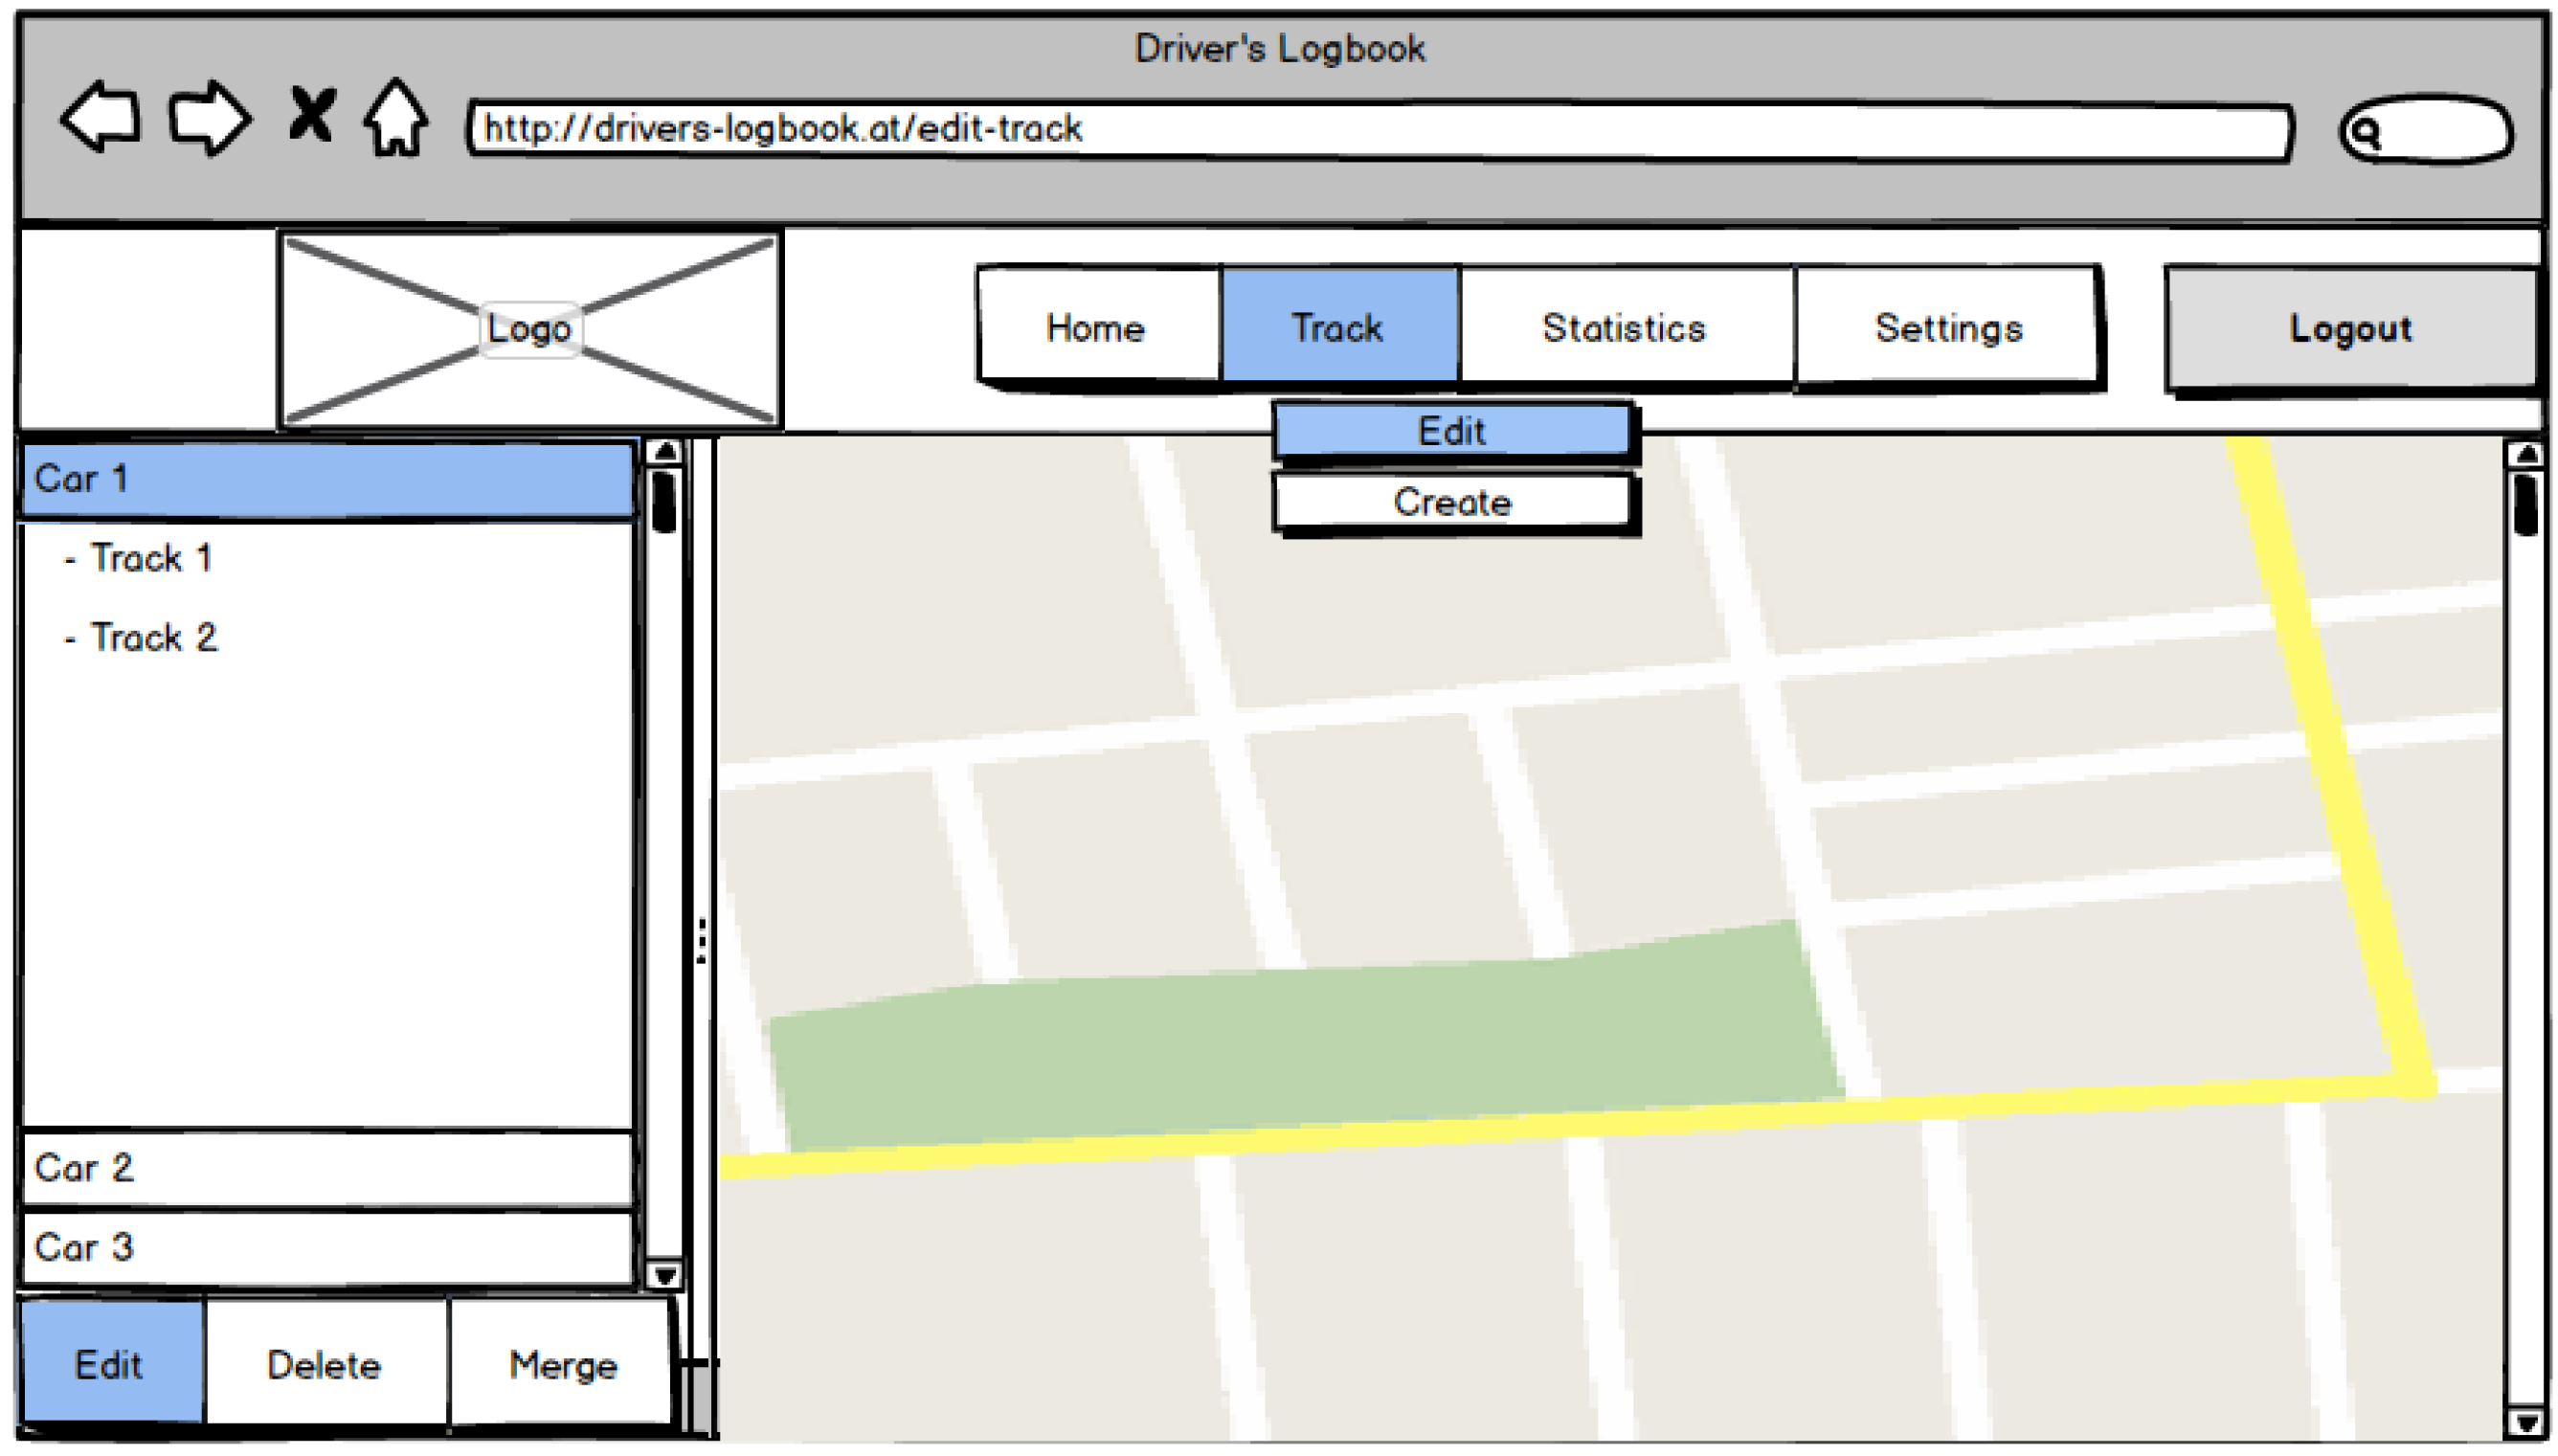
\includegraphics[width=1\textwidth]{bilder/WebPortal}
\end{center}
